\section{Silizium-PVD}
\label{siliconpvd}

\todoline{Jörg}
Die Abscheidung amorpher Strukturen für durch Silizium-PVD soll unter Nutzung reaktiver Kraftfelder mit Parsivald simuliert werden.
Nach Voruntersuchungen verschiedener ReaxFF-Para\-metrisierungen werden Abscheidungen auf kristallinen Silizium-Substraten unterschiedlicher Schnittebenen simuliert, die gleichartiges Wachstum zeigen, welches anhand einer ausgewählten Struktur untersucht wird.
Anschließend werden Simulationen von Reaktionen der Siliziumdioxid-Precursor \ce{SiH4} und \ce{O2} präsentiert, welche zur \ce{SiO2}-CVD hinführen sollen.

\subsection{Potentialdateien}

\todoline{Neu schreiben: Kausalität beachten! Silizium -> gerichtete Bindungen -> Reax -> amorph}
Die Wahl fiel dabei auf ReaxFF-Formulierungen, um neben EAM-Kraftfeldern, welche scheinbar epitaktisches Wachstum bevorzugen, auf eine Methode zurück zu greifen, die durch die Formulierung von Bindungsordnungen die Silizium-Atome an ihre Nachbarn bindet und so durch verminderte Mobilität amorphe Strukturen erzeugt.
Da die ReaxFF-Formulierung erst innerhalb des letzten Jahrzehntes an Popularität gewonnen hat, sind die verfügbaren Potentiale auf einzelne Probleme angepasst und oftmals noch nicht in den Potentialdatenbanken zu finden.
Tabelle~\ref{tab:siliconpotentials} listet die im Rahmen der Arbeit untersuchten ReaxFF-Parametrisierungen auf.

Zudem lohnt sich die Untersuchung der ReaxFF-Parametrisierungen im Hinblick auf die Darstellbarkeit von Silan und Wasser sowie deren Reaktionen mit einander und mit Siliziumdioxid-Oberflächen, womit die umfassende Simulation eines CVD-Prozesses ermöglicht würde.

\begin{table}[hb]
  \caption{Untersuchte ReaxFF-Parametrisierungen für Silizium- und Siliziumoxidsysteme}
  \label{tab:siliconpotentials}
  \oddrowcolors
  \begin{tabularx}{1\textwidth}{|lXc|}
    \hline
    \textbf{Bezeichnung} & \textbf{Anwendung \& Kommentare}                                                                          & \textbf{Ref.}                     \\
    \hline
    Al\_AlO\_AlN         & \ce{Al}, \ce{Al2O3}, \ce{AlN}. Basiert auf einer Si-Parametrisierung                                      & \cite{plimpton_lammps_2014}       \\
    chenoweth            & Zersetzung von Polydimethylsiloxane bei hohen Drücken und Temperaturen. Ergänzung von \ce{C-Si}-Bindungen & \cite{chenoweth_simulations_2005} \\
    kulkarni             & Reaktion von Sauerstoff mit \ce{OH}-terminierten Siliziumoxid-Oberflächen                                 & \cite{kulkarni_oxygen_2013}       \\
    lg                   & ``low gradients''. Siehe liu\_nitramines. Fehlerhafte Version aus LAMMPS                                  & \cite{liu_reaxff-lg:_2011}        \\
    liu\_ettringite      & Verspannung von Ettringit (\ce{Ca6[Al(OH)6]2(SO4)3 26H2O}). Basiert auf Si-Parametrisierung               & \cite{liu_development_2012}       \\
    liu\_nitramines      & Dichtebestimmung von Nitramin-Molekülen bei hohen Drücken. Dichte erhöht durch Van-der-Waals-Korrekturen  & \cite{liu_reaxff-lg:_2011}        \\
    narayanan            & Präparation mit \ce{Li-Al}-Silikaten. Für Phasenübergänge von Eukryptit-Kristallen (\ce{LiAl[SiO4]})      & \cite{narayanan_reactive_2012}    \\
    newsome              & Oxidation von \ce{SiC}-Oberflächen mit \ce{O2} und \ce{H2O} bei \SIrange{500}{5000}{\kelvin}              & \cite{newsome_oxidation_2012}     \\
    nielson              & Reaktionskinetik an Metallkatalysatoren bei hohen Temperaturen                                            & \cite{nielson_development_2005}   \\
    zhang                & Zersetzung energetischer Moleküle (Nitramin-Explosionen)                                                  & \cite{zhang_carbon_2009}          \\
    \hline
  \end{tabularx}
\end{table}

\subsection{Voruntersuchungen}

In Ergänzung zu den bisherigen Voruntersuchungen, die hauptsächlich aus Optimierungen und Relaxierungen von Kristallen bestanden, kommen hier auch Simulationen der Oberfläche und der amorphen Struktur hinzu, wie sie bereits in Abschnitt~\ref{mdmethods} vorgestellt wurden.
Diese zusätzlichen Untersuchungen haben umfassendere Aussagen über die Anwendbarkeit der Parametrisierungen für vollständige Abscheidungssimulationen zum Ziel.
Die Ergebnisse dieser Betrachtungen wurden in Tabelle~\ref{tab:siliconpreresults} zusammen gefasst und werden im Weiteren kurz diskutiert.

\begin{table}
  \begin{threeparttable}
    \caption[Zusammenfassung der Voruntersuchungen für Silizium-Systeme]{
      Zusammenfassung der Voruntersuchungen für Silizium-Systeme.
      Siehe Anhang~\ref{appendix:silicon}
    }
    \label{tab:siliconpreresults}

    \oddrowcolors
    \begin{tabularx}{\textwidth}{|lCCCCCCC|}
      \hline
      \textbf{Bezeichnung}    & LMP\tnote{a}    & c-\ce{Si} & c-\ce{SiO2} & a-\ce{Si} & \ce{SiH4} & \ce{+O2} & PVD\tnote{b} \\
      \hline                % & LAMMPS & c-Si      & c-SiO2      & a-Si      & Silane    & +O2      & PVD          \\
      Al\_AlO\_AlN            & \cmark & ~         & (\cmark)    &  \cmark   & \cmark    & ~        & \cmark       \\
      chenoweth               & ~      & ~         & ~           &  ~        & ~         & ~        & ~            \\
      kulkarni                & \cmark & \cmark    & \cmark      &  \cmark   & \cmark    & (\cmark) & \cmark       \\
      lg                      & ~      & ~         & ~           &  ~        & ~         & ~        & ~            \\
      liu\_ettringite         & \cmark & ~         & \cmark      &  \cmark   & ~         & ~        & \cmark       \\
      liu\_nitramines         & ~      & ~         & ~           &  ~        & ~         & ~        & ~            \\
      narayanan               & \cmark & ~         & \cmark      &  \cmark   & ~         & ~        & \cmark       \\
      newsome                 & \cmark & ~         & (\cmark)    &  ~        & ~         & (\cmark) & \cmark       \\
      nielson                 & \cmark & \cmark    & \cmark      &  \cmark   & \cmark    & ~        & \cmark       \\
      zhang                   & \cmark & ~         & ~           &  ~        & \cmark    & \cmark   & ~            \\
      \hline
    \end{tabularx}

 %% & CVD\tnote{b}
 %% & CVD
 %% & \cmark?
 %% & ~
 %% & \cmark?
 %% & ~
 %% & \cmark?
 %% & ~
 %% & \cmark?
 %% & \cmark?
 %% & \cmark?
 %% & ~

    \begin{tablenotes}[para]
      \item[a] LMP: Kompatibilität mit LAMMPS
      \item[b] PVD: a-\ce{Si}-PVD mit Parsivald
      %% \item[b] CVD: a-\ce{SiO2}-CVD mit Parsivald
    \end{tablenotes}
  \end{threeparttable}
\end{table}

\subsubsection{Kompatibilität mit der Molekulardynamiksoftware (LMP)}

Einige Potentialdateien sind aus verschiedenen Gründen nicht mit der aktuellen Version der LAMMPS-Bibliothek kompatibel, was sich in harten Abbrüchen des Programmes äußert und sie von weiteren Untersuchungen ausschließt.
\todo{Fußnote verständlich machen}Andere Dateien lassen sich zwar laden und benutzen, äußern jedoch regelmäßige Warnungen über ihre van-der-Waals-Parameter, die aber nicht zu sonstigen Fehlern führen und meist nur Stickstoff- oder Platzhalteratome\footnote{Typischerweise beinhalten ReaxFF-Dateien wechselwirkungsfreie Platzhalterelemente unter dem Platzhalter-Element \ce{X} zur Festlegung wechselwirkungsfreier Atome in der Simulation} betrifft.

\subsubsection{Kristalleigenschaften (c-\ce{Si}, c-\ce{SiO2})}

\todo{``decken sich''}Diese Untersuchungen, deren Ergebnisse detailliert in Anhang~\ref{appendix:silicon} dargestellt sind, decken sich mit dem bisherigen Vorgehen:
Eine Kristallstruktur wird unterhalb des Schmelzpunktes relaxiert, minimiert und anschließend hinsichtlich Koordination, Dichte und Bindungslänge analysiert.
Alle untersuchten Parametersätze erzeugen die korrekte Koordinationszahl von 4.0, mit klaren Spitzen in den radialen Verteilungsfunktionen und nahezu passenden Bindungslängen (Abbildung~\ref{fig:sisibondlengths}).
Der Newsome-Parametersatz generiert einen RDF-Peak vor der eigentlichen Bindungslänge, welcher der Vollständigkeit halber erwähnt sein soll, bei Bestimmung der Bindungslänge aus der RDF aber nicht über die Hauptbindungslänge dominiert.
Er führt bei amorphen Systemen jedoch zu einer Unterschätzung der Bindungslänge und Koordinationszahl (Tabelle~\ref{tab:amorphoussilicon}).
Im Allgemeinen stimmen die Kristalleigenschaften gut mit den erwarteten Werten aus der \todo{Ref}Literatur überein.
Anhang~\ref{appendix:silicon} beinhaltet Abbildungen eines Vergleiches der Bindungslängen sowie eine exemplarische radiale Verteilungsfunktion des Kulkarni-Potentiales im kanonischen und im isotherm-isobaren Ensemble.

\subsubsection{Amorphes Silizium (a-\ce{Si})}

Durch langsame Relaxation zufällig positionierter Siliziumatome wurde amorphes Silizium simuliert, das wie die Kristalle zuvor auf Dichte und Bindungslängen untersucht wurde.
Deren Werte variieren für amorphes Silizium stärker als für kristallines, liegen jedoch nah am experimentell bestimmten Wert von \SI{2.3}{\gpcc}\cite{remes_optical_1998}.

\subsubsection{Abscheidungssimulationen (PVD)}

Die Abscheidungssimulationen selbst verlaufen wie in Kapitel~\ref{parsivald} vorgestellt und unterscheiden sich kaum von den Parsivald-Simulationen der vorherigen Abschnitte.
\todo{Nein! Nicht durch die Kraftfelder!}Durch die reaktiven Kraftfelder werden kompliziertere lokale Bindungsverhältnisse erwartet, die zu amorphen und damit rauheren Strukturen führen.
%Als Ausgang werden amorphe und deshalb rauhere Schichten erwartet, die sowohl für \ce{Si}-PVD als auch \ce{SiO2}-CVD kontinuierlich wachsen, aber unterschiedlichen Bedingungen unterliegen.

\subsection{Silizium-PVD}

Silizium-PVD dient in der Produktion elektronischer Bauelemente der Erzeugung einer dünnen, amorphen Siliziumschicht für unterschiedliche Anwendungsszenarien\todo{welche Anwendungen für a-Si? Solarzellen?}, für die konforme Schichten gleichbleibender Qualität gewünscht sind.
Durch den amorphen Charakter des Materials sind nanoskopische Leerstellen und höhere Rauheiten als bei monokristallinen Schichten zu erwarten, die im Folgenden kurz untersucht werden sollen.
\todo{Felix schreibt so was auch, wenn er keinen besseren Ausdruck findet.}Rechenaufwendigere Rechenvorschriften des ReaxFF-Potentiales legen eine längere Simulationsdauer als bei EAM-Potentialen nahe, weshalb nur eine kleine Menge an Simulationen durchgeführt wurde.
Typische Laufzeiten von mehreren Wochen wurden für vollständige ReaxFF-Abscheidungssimulationen beobachtet, jedoch sind im Gegensatz zu rein molekulardynamischen Untersuchungen größere Simulationsräume mit isolierten Ereignissen möglich, die eine Reduktion einiger Finite Size-Effekte zur Folge hat.

Als Substrat für die Parsivald-Simulationen wurden unrelaxierte Silizium-Monokristalle mit Oberflächen entlang der drei Kristallebenen (001), (011) und (111) präpariert und durch periodische Erweiterung auf \SI{106.416x103.68}{\angstrom} vergrößert.
Sonstige Parameter umfassen eine Temperatur von \SI{1300}{\kelvin} (der Schmelzpunkt liegt bei \SI{1687}{\kelvin}), Relaxationszeiten von \SI{350}{\femto\second} und MD-Box-Größen von \SI{37x37}{\angstrom}.
Die Auftreffenergie der Silizium-Atome liegt mit \SI{11.2}{\electronvolt} erneut vergleichsweise hoch, wird aber auch hier durch das Thermostat auf einen unbestimmten Wert verringert.
Damit werden im Schnitt \num{1.68} parallele Ereignisse mit durchschnittlich \num{1510.65} Atomen und einer mittleren Laufzeit von \SI{60.71}{\second} berechnet.
Die Laufzeit lässt sich beispielsweise über die Zeitschrittweite noch minimieren, zeigt allerdings den Unterschied in der Laufzeit bei der Nutzung von EAM- und ReaxFF-Potentialen, der einem Faktor von etwa \num{12} für vergleichbare Simulationen entspricht.
Die hohe Temperatur wurden zur Beschleunigung der Relaxationen gewählt und übersteigt die Temperaturen realer Abscheidungen.
Durch Optimierung der Simulation durch Relaxationszeit, Zeitschrittweite, Thermostatdämpfung und Teilchenenergie ließe sich die Temperatur auf einen realistischeren Wert bei gleicher Verlässlichkeit der Simulation senken.

Das Ergebnis der Abscheidungssimulation ist eine vergleichsweise glatte, amorphe Siliziumschicht, die mit konstanter Rate wächst, jedoch eine Zunahme der Rauheit aufgrund von sich langsam verstärkenden Oberflächenunebenheiten aufweist.

Zur Charakterisierung der Kristalleigenschaften der abgeschiedenen Schicht wurden ihre radiale Verteilungsfunktionen berechnet, aus denen ersichtlich ist, dass bereits nach \SI{4}{\angstrom}, also kurz vor der zweiten Korrelationslänge bei \SI{4.4}{\angstrom}, keine langreichweitige Ordnung mehr vorhanden ist.
Die engen Spitzen an den charakteristischen Abständen des reinen Silizium-Kristalles werden durch das Substrat erzeugt\todo{Schicht ohne Substrat RDF-untersuchen}, welches bei \SI{100}{\angstrom} Schichtdicke immerhin noch \SI{20}{\percent} der Struktur ausmacht, jedoch durch anfängliche Relaxierungen zum Teil seine Kristalleigenschaften verloren hat.
Anders als bei Gold oder Kupfer, bei denen metallische Bindungen dominieren, überwiegen in reinem Silizium kovalente Bindungen, so dass die mittleren Koordinationszahl von \num{3.99} anzeigt, dass alle 4 möglichen Bindungen der Siliziumatome tatsächlich ausgeprägt sind.
Somit zeigt sich die ReaxFF-Formulierung erfolgreich in der Darstellung der strukturellen Eigenschaften von Silizium.

\todoline{Anhang-Referenzen vermindern}
Die Unebenheiten der Schicht, welche die Form von Nanoporen annehmen, wachsen im Gegensatz zu den Kupfer-Kratern aus Abschnitt~\ref{copperpvd} mit der Oberfläche entlang der Wachstumsrichtung, schließen sich aber ebenfalls selbsttätig, wenngleich über einen größeren Zeitraum.
Abbildung~\ref{fig:siliconresults-a} stellt dazu über der Simulationszeit neben der Schichtdicke die Rauheit dar, welche im Verlauf der Simulation linear steigt und zuletzt einen RMS-Wert von \SI{1.15}{\nano\meter} annimmt, der experimentellen Erwartungen von \SIrange{1}{10}{\nano\meter} entspricht\cite{gago_nanopatterning_2002}.
An Abbildung~\ref{fig:siliconroughness} lässt sich erkennen, dass die Rauheit \todo{weiter schreiben}asd
\todo{Leider?}Leider ermöglicht die begrenzte Laufzeit der Simulation keine Aussage über den weiteren Verlauf der Rauheit, von der sublinearer Verlauf durch Schließung der Unebenheiten erwartet wird, wie er sich bei Sputterprozessen zeigt\cite{gago_nanopatterning_2002}\todo{Hinweis auf nicht-sublinearen Verlauf!}.

\begin{figure}
  \captionsetup[subfigure]{singlelinecheck=false}
  \def\subfigwidth{0.48\textwidth}
  \begin{subfigure}[t]{\subfigwidth}
    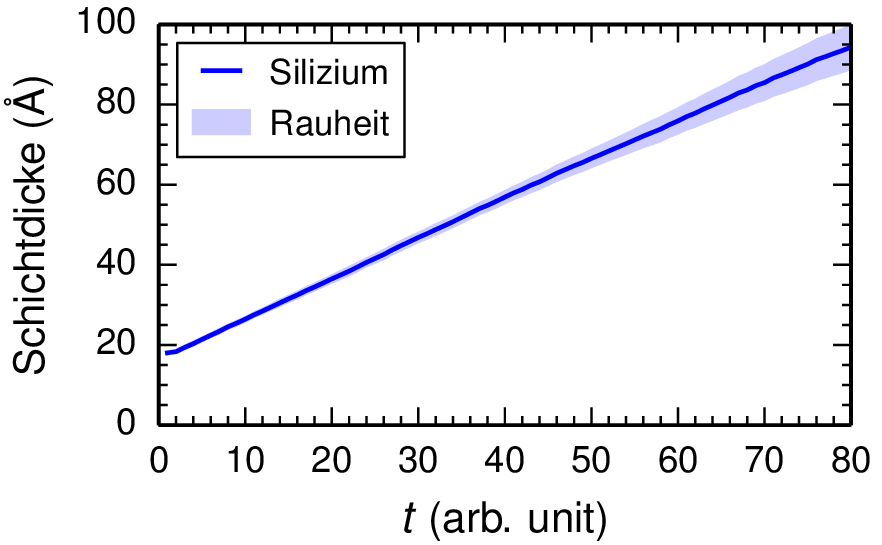
\includegraphics[width=\textwidth]{Si111_combined}
    \subcaption{Dicke und Rauheit der Schicht}
    \label{fig:siliconresults-a}
  \end{subfigure}
  \hfill
  \begin{subfigure}[t]{\subfigwidth}
    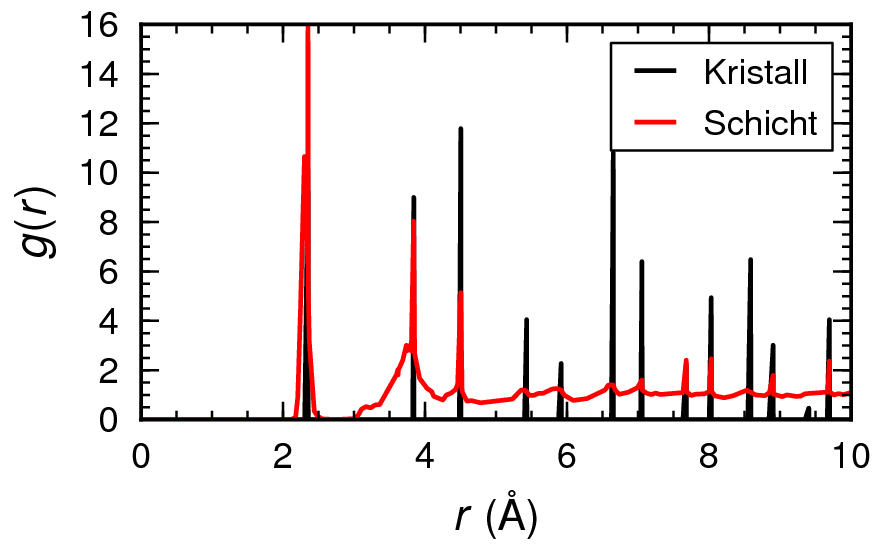
\includegraphics[width=\textwidth]{si111_rdf}
    \subcaption{Radiale Verteilungsfunktion bei $t=80$}
    \label{fig:siliconresults-b}
  \end{subfigure}
  \caption[Struktur einer Silizium-PVD-Schicht aus Parsivald]{
    Struktur einer Silizium-PVD-Schicht aus Parsivald (\SI{10x10}{\nano\meter})
  }
  \label{fig:siliconresults}
\end{figure}

Abbildung~\ref{fig:siliconprofile} stellt die räumliche Verteilung der Unebenheiten dar, die sich lokal in Kratern und Poren von bis zu \SI{32}{\angstrom} Tiefe konzentrieren, aufgrund ihrer geringen Breite aber nur zu einer RMS-Rauheit von \SI{11.5}{\angstrom} führen.
Breitere Krater haben sich durch die geringe Größe des Simulationsraumes nicht entwickelt, jedoch wäre eine Untersuchung einer ca. \SI{500x500}{\angstrom} breiten Struktur auf deren Bildung interessant.
Anhand des Profiles lässt sich auch erkennen, dass mitunter längere Relaxationszeiten oder höhere Teilchenenergien notwendig wären, um Porenbildung weiter zu verringern und langreichweitigere Unebenheiten zu befördern, wie sie etwa bei der Bildung nanoskopischer Silizium-Partikel auftreten würden.

Zum Vergleich beinhaltet Abbildung~\ref{fig:siliconunderrelaxedprofile} das Oberflächenprofil einer unterrelaxierten Oberfläche, wie sie während der Anpassung der Parsivald-Parameter entstanden sind.
Es zeigen sich stärkere Unterschiede und steilere Hänge, die sich aus der hohen Porösität des Materiales ergeben.
Die Porentiefen betragen \SI{6}{\nano\meter} und wachsen linear mit der Schichtdicke, wobei sich aus Zählung der Atome und des Volumens eine Dichte von \SI{2.634}{\gpcc} ergibt, welche durch die Unterschätzung der mittleren Höhe der Oberfläche durch die Nanoporen etwas überschätzt wird und somit oberhalb der kristallinen Dichte von \SI{2.32}{\gpcc} liegt.
Somit ist zu erwarten, dass die Rauheit der Schicht mit stärkerer Relaxierung während der Abscheidung weiter abnimmt.

\begin{figure}[H]
  \centering
  \captionsetup[subfigure]{singlelinecheck=false}
  \begin{subfigure}[t]{7.1cm}
    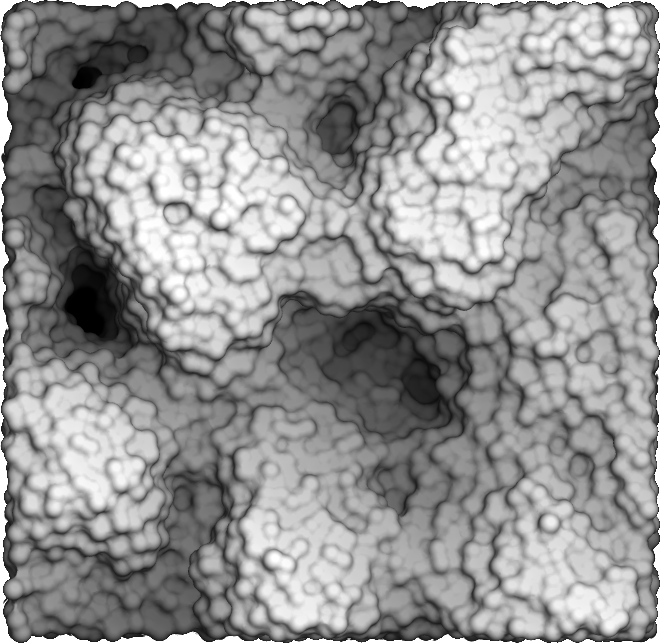
\includegraphics[width=\textwidth]{si111_surface_profile}
  \end{subfigure}
  \begin{subfigure}[t]{1.7cm}
    \def\svgwidth{\textwidth}
    \begin{overpic}[width=0.7cm]{greyhalfscale}
      \put(0,0){\input{img/si111_surface_profile_halfscale.pdf_tex}}
    \end{overpic}
  \end{subfigure}
  \caption[Oberflächenprofil einer Silizium-PVD-Schicht]{
    Oberflächenprofil einer auf Si-(111) per PVD abgeschiedenen Schicht
  }
  \label{fig:siliconprofile}
\todoline{Längenskala}
\end{figure}

\begin{figure}[H]
  \centering
  \captionsetup[subfigure]{singlelinecheck=false}
  \begin{subfigure}[t]{7.1cm}
    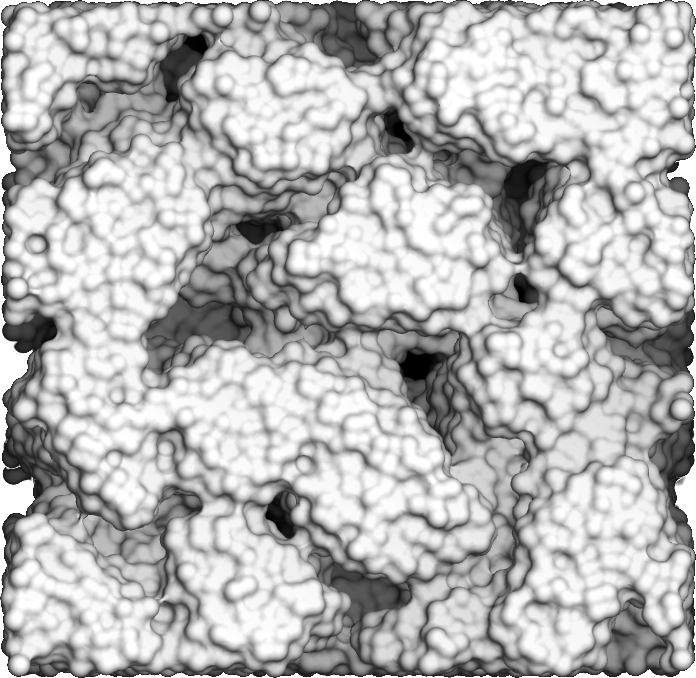
\includegraphics[width=\textwidth]{si111_underrelaxed_profile}
  \end{subfigure}
  \begin{subfigure}[t]{1.7cm}
    \def\svgwidth{\textwidth}
    \begin{overpic}[width=0.66cm]{greyscale}
      \put(0,0){\input{img/si111_underrelaxed_profile_scale.pdf_tex}}
    \end{overpic}
  \end{subfigure}
  \caption[Oberflächenprofil einer unterrelaxierten Siliziumschicht]{
    Oberflächenprofil einer unterrelaxierten, porösen Silizium-PVD-Schicht
  }
  \label{fig:siliconunderrelaxedprofile}
\end{figure}

\subsection{Voruntersuchungen für Siliziumdioxid-CVD}

ReaxFF-Potentiale versprechen die Simulation von Molekülen und deren Reaktion miteinander, die mit den folgenden Tests für Silan und molekularen Sauerstoff überprüft werden sollen.

\subsubsection{Stabilität der Precursormoleküle (\ce{SiH4}, \ce{O2})}

Simulationen einzelner und mehrerer Precursormoleküle (\ce{SiH4} und \ce{O2}) hinsichtlich ihrer Stabilität wurden im mikrokanonischen beziehungsweise kanonischen Ensemble bei verschiedenen Temperaturen durchgeführt.
\todo{Abbildung hier her kopieren}Abbildung~\ref{fig:silanestability} zeigt eine Auswahl der Ergebnisse der Silan-Simulationen, an denen sich erkennen lässt, wie instabile Simulationen zur Ablösung der Wasserstoffatome vom Silanmolekül führen.

\subsubsection{Reaktion der Precursormoleküle (\ce{SiH4 + O2})}

Reaktionen von einzelnen Precursormolekülen wurden stichprobenartig in verschiedenen Orientierungen, Energien und Temperaturen vorgenommen, um einen Überblick über die Verlässlichkeit zu bekommen.
Zusätzlich wurden durchmischte Precursorgase mit dem Ziel eventueller Reaktionen simuliert, was jedoch mit keiner der Parametrisierungen zum gewünschten Erfolg bei hoher Zuverlässigkeit führte.
Einige Parametrisierungen zeigen jedoch vielversprechende Teilreaktionen, die korrekte Doppelbindungen und Bildung von Wasserstoffmolekülen beinhalten (\todo{Abbildung hier her kopieren}Abbildung~\ref{fig:precursorreactions}).
Vor allem bei größeren Reaktionsräumen bilden sich Cluster aus Precursormolekülen, die von attraktiven Termen in den Kraftfeldern dominiert werden, aber nicht durch chemische Wechselwirkungen zu erklären sind (\todo{Abbildung hier her kopieren}Abbildung~\ref{fig:precursorclusters}).

